\documentclass[11pt]{article}

\usepackage[a4paper,margin=2.5cm]{geometry}
\usepackage{amsmath,amssymb,amsthm}
\usepackage{graphicx}
\usepackage{booktabs}
\usepackage{array}
\usepackage{xcolor}
\usepackage{enumitem}
\usepackage{hyperref}
\hypersetup{colorlinks=true,linkcolor=blue!50!black,urlcolor=blue!50!black}

\newcommand{\state}[1]{\texttt{(#1)}}
\newcommand{\empt}{\texttt{(\,)}}
\newcommand{\R}{\mathbb{R}}
\newtheorem{definition}{Definition}
\newtheorem{remark}{Remark}

\title{\textbf{A Complete, Certified Search for Stationary\\ Markov Perfect Equilibria in Farsighted Coalition Formation}\\[4pt]
\large Strategy document --- worked through the \texttt{burke\_usaruschn\_2035--2060} instance}
\author{}
\date{\today}

\begin{document}
\maketitle

\begin{abstract}
This document lays out, step by step, the strategy we intend to pursue for
\emph{certifiably} finding a stationary Markov Perfect Equilibrium (MPE) of the
farsighted coalition-formation game, or characterising why doing so is hard. It is
written to be judged: before committing weeks or months of compute, we want the
mathematics and the combinatorial accounting to be transparent and correct. Every
abstract object (player, state, transition, committee, weak order, ``degeneracy'')
is illustrated on one concrete instance, the payoff table
\texttt{burke\_usaruschn\_2035--2060.xlsx}, which we have selected as the running
example and first target. We are explicit about where a number is an exact count and
where it is a (possibly loose) upper bound, because an earlier version of our own
reasoning conflated the two.
\end{abstract}

\tableofcontents

\section{The game instance}
\label{sec:game}

\subsection{Players and the running example}
The game has $n=3$ players. In the running instance they are the economic blocs
\textbf{CHN}, \textbf{RUS}, \textbf{USA}. Each may participate in a coalition that
deploys solar geoengineering (SG). The instance is defined by a payoff table; its
contents are shown in Figure~\ref{fig:table}.

\begin{figure}[h]
\centering
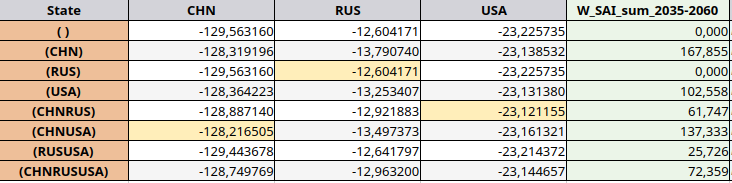
\includegraphics[width=\textwidth]{burke_usaruschn_2035-2060_screenshot.png}
\caption{The payoff table \texttt{burke\_usaruschn\_2035--2060}. Each row is a
coalition structure; the columns \textbf{CHN}, \textbf{RUS}, \textbf{USA} give the
static payoff $u_i(x)$ to each player in that structure, and the last column is the
implied SG deployment level $G$. Payoffs are (negative) economic outcomes, so larger
(less negative) is better.}
\label{fig:table}
\end{figure}

\subsection{States (coalition structures)}
\label{sec:states}
A \emph{state} is a coalition structure: who cooperates with whom. The table lists
eight rows, but under the \emph{power-threshold} governance rule a single country
cannot deploy SG (it lacks the required power share, here $\geq 50.1\%$ with equal
power $1/3$ each). Hence the three singleton rows \state{CHN}, \state{RUS},
\state{USA} are payoff-identical to the no-cooperation state \empt{} --- indeed in
Figure~\ref{fig:table} the rows \empt{}, \state{RUS} and the deployment column all
read $G=0$. The framework therefore collapses to the
\textbf{$S=5$ canonical states}:
\[
\mathcal{X} = \{\ \empt,\ \state{CHNRUS},\ \state{CHNUSA},\ \state{RUSUSA},\ \state{CHNRUSUSA}\ \}.
\]
Concretely \state{CHNRUS} is ``CHN and RUS cooperate and jointly deploy; USA is
alone,'' and \state{CHNRUSUSA} is the grand coalition. The static payoff matrix
$u_i(x)$ we actually use (extracted from the table) is

\begin{table}[h]
\centering
\begin{tabular}{lrrrr}
\toprule
state $x$ & $u_{\text{CHN}}(x)$ & $u_{\text{RUS}}(x)$ & $u_{\text{USA}}(x)$ & $G(x)$\\
\midrule
\empt        & $-129.563160$ & $-12.604171$ & $-23.225735$ & $0.000$\\
\state{CHNRUS}    & $-128.887140$ & $-12.921883$ & $-23.121155$ & $61.747$\\
\state{CHNUSA}    & $-128.216505$ & $-13.497373$ & $-23.161321$ & $137.333$\\
\state{RUSUSA}    & $-129.443678$ & $-12.641797$ & $-23.214372$ & $25.726$\\
\state{CHNRUSUSA} & $-128.749769$ & $-12.963200$ & $-23.144657$ & $72.359$\\
\bottomrule
\end{tabular}
\caption{The five-state payoff matrix used by the solver, with deployment levels.}
\label{tab:payoffs}
\end{table}

\subsection{Timing, protocol, discounting}
Time is discrete. In each period one player is drawn as \emph{proposer} according to
a fixed protocol $\rho$; here it is uniform, $\rho_{\text{CHN}}=\rho_{\text{RUS}}=
\rho_{\text{USA}}=\tfrac13$. The chosen proposer may propose moving to a different
state; an \emph{approval committee} then votes; if it approves, the system moves,
otherwise it stays. Future payoffs are discounted by $\delta=0.99$.

\subsection{Which transitions are allowed: the effectivity rule \texttt{adjacent\_step}}
\label{sec:adjacency}
Not every state-to-state move can be proposed. We use the effectivity rule
\texttt{adjacent\_step}: a proposer may only propose a move that changes the
deploying coalition by \emph{one membership event} (one country joins, or one
leaves, or a pair forms/dissolves). Concretely, for the running instance the allowed
(non-forbidden) moves form a ``diamond'':
\[
\empt \;\longleftrightarrow\; \{\,\state{CHNRUS},\,\state{CHNUSA},\,\state{RUSUSA}\,\}
\;\longleftrightarrow\; \state{CHNRUSUSA},
\]
plus the self-loop ``stay'' at every state. That is:
\begin{itemize}[nosep]
\item From \empt{} one may form any pair, e.g.\ \empt$\to$\state{CHNRUS}, but
\textbf{not} jump straight to the grand coalition (\empt$\to$\state{CHNRUSUSA} is
\emph{forbidden} --- that would be two events).
\item From a pair, e.g.\ \state{CHNRUS}, one may dissolve to \empt{} or admit the
third member to reach \state{CHNRUSUSA}; one may \textbf{not} jump to another pair
(\state{CHNRUS}$\to$\state{CHNUSA} is forbidden --- RUS leaves \emph{and} USA joins).
\item From the grand coalition one member may leave (\state{CHNRUSUSA}$\to$
\state{CHNRUS}); all three dissolving at once (\state{CHNRUSUSA}$\to$\empt) is
forbidden.
\end{itemize}
Counting allowed targets (including ``stay'') per state gives
\[
\#\text{feasible}(\empt)=4,\quad \#\text{feasible}(\text{pair})=3\ \text{(each)},\quad
\#\text{feasible}(\state{CHNRUSUSA})=4 .
\]
We write $\mathcal{F}(i,x)$ for the set of states proposer $i$ may propose from $x$;
under this rule it does not depend on $i$, so e.g.\ $\mathcal{F}(\cdot,\empt)=
\{\empt,\state{CHNRUS},\state{CHNUSA},\state{RUSUSA}\}$. \texttt{adjacent\_step} is
deliberately restrictive: fewer feasible transitions means smaller approval
committees and a smaller search, which is exactly why we prefer it over the looser
2021 rule.

\subsection{Who must approve: committees}
\label{sec:committees}
For each potential move ``proposer $i$ proposes $x\to y$'' the governance structure
fixes an \emph{approval committee} $C(i,x,y)\subseteq\{$CHN,RUS,USA$\}$ whose consent
is required (unanimously, since \texttt{unanimity\_required} is true here). These are
fixed rules, \emph{not} decision variables. Examples from the running instance:
\begin{itemize}[nosep]
\item CHN proposes \empt$\to$\state{CHNRUS}: committee $=\{$RUS$\}$ (CHN wants in; RUS
must consent to pair with CHN; USA is unaffected).
\item CHN proposes \empt$\to$\state{RUSUSA}: committee $=\{$RUS,USA$\}$ (CHN proposes
a coalition it is \emph{not} part of; both members must consent).
\item CHN proposes \state{CHNRUSUSA}$\to$\state{RUSUSA} (CHN exits the grand
coalition): committee $=\{$CHN$\}$ --- a country may leave unilaterally.
\end{itemize}

\section{Strategies}
\label{sec:strategies}
A (stationary, Markov) strategy profile $\sigma$ specifies two kinds of behaviour.

\paragraph{Proposal probabilities.} For each proposer $i$ and current state $x$, a
probability distribution over feasible next states:
$\sigma^P_i(x,\cdot)$ on $\mathcal{F}(i,x)$, summing to $1$. Example: ``when USA is
drawn in state \state{CHNRUS}, it proposes \state{CHNRUSUSA} with probability $1$''
is the pure proposal $\sigma^P_{\text{USA}}(\state{CHNRUS},\state{CHNRUSUSA})=1$.

\paragraph{Acceptance probabilities.} For each committee member $k\in C(i,x,y)$, the
probability $\sigma^A_k(x,y\mid i)\in[0,1]$ that $k$ votes to approve. Only committee
members have a decision; others are undefined. Example: in the move
CHN proposes \empt$\to$\state{CHNRUS}, the only decision is RUS's accept probability.

We index an acceptance decision by the quadruple $(i,x,y,k)$: \emph{proposer} $i$,
\emph{from} $x$, \emph{to} $y$, \emph{approver} $k$. We call $(i,x,y,k)$ a
\emph{context}. The same underlying preference of $k$ (does $k$ like $y$ better than
$x$?) can appear in several contexts (different proposers $i$), which will matter for
variable elimination in Section~\ref{sec:comp-r}.

\section{Value functions and the equilibrium conditions}
\label{sec:mpe}

\subsection{Continuation values}
A profile $\sigma$ induces a transition matrix $P=P(\sigma)$ on the five states: the
probability of moving $x\to y$ in one period, obtained by summing over who is drawn
($\rho_i$), what they propose ($\sigma^P$), and whether the committee approves
($\prod_{k\in C}\sigma^A_k$, by unanimity). Given $P$, the long-run value to player
$i$ in state $x$ solves the Bellman equation
\begin{equation}
\label{eq:bellman}
V_i(x) = (1-\delta)\,u_i(x) + \delta \sum_{y} P(x,y)\,V_i(y),
\qquad\text{i.e.}\qquad
V_i = (I-\delta P)^{-1}(1-\delta)\,u_i .
\end{equation}
Crucially, $P(\sigma)$ is a \emph{multilinear} (hence polynomial) function of the
strategy probabilities, and $V$ is therefore a \emph{rational} function of $\sigma$
(ratios of determinants). This polynomial structure is what later makes exact,
certified solving possible in principle.

\subsection{The two rationality conditions}
A profile is a stationary MPE iff, simultaneously:
\begin{description}
\item[(A) Approval rationality.] A committee member approves iff the destination
improves its own value:
\[
\sigma^A_k(x,y\mid i) =
\begin{cases}
1 & \text{if } V_k(y) > V_k(x),\\
0 & \text{if } V_k(y) < V_k(x),\\
\text{any value in }[0,1] & \text{if } V_k(y) = V_k(x).
\end{cases}
\]
\item[(P) Proposal rationality.] A proposer puts positive probability only on moves
that maximise its expected continuation value, accounting for the chance of approval:
\[
\sigma^P_i(x,y)>0 \ \Longrightarrow\
y \in \arg\max_{y'\in\mathcal{F}(i,x)}
\Big[\,p^A(i,x,y')\,V_i(y') + \big(1-p^A(i,x,y')\big)V_i(x)\,\Big],
\]
where $p^A(i,x,y')=\prod_{k\in C(i,x,y')}\sigma^A_k(x,y'\mid i)$ is the committee
approval probability and the bracket is the \emph{expected value} $\mathrm{EV}$ of
proposing $y'$.
\end{description}
The difficulty is the coupling: $\sigma$ determines $P$, which determines $V$ via
\eqref{eq:bellman}, which determines what is rational in (A) and (P), which
determines $\sigma$. An equilibrium is a fixed point of this loop. Existence is not
in doubt: Fink's theorem guarantees that every finite discounted stochastic game has
at least one stationary equilibrium in behavioural (mixed) strategies. The problem is
\emph{finding} one, with certainty.

\section{Reduction to ordinal rankings, and the $541^3$ count}
\label{sec:ordinal}

\subsection{Why only the ordering of $V$ matters}
Inspect conditions (A) and (P): both depend on $V$ \emph{only through comparisons}.
Condition (A) asks whether $V_k(y)$ is greater than, less than, or equal to
$V_k(x)$. Condition (P) asks which $y'$ \emph{maximises} an expression; away from
ties, the maximiser is determined by the order of the relevant values. Therefore the
\emph{qualitative} equilibrium behaviour is fixed once we know, for each player, the
\textbf{ordinal ranking} of the five continuation values $V_k(\empt),\dots,
V_k(\state{CHNRUSUSA})$.

\subsection{Strict orders, weak orders, and the count}
For one player there are $S=5$ states. If all five values are distinct, the ranking
is a \emph{strict total order} --- a permutation --- and there are $5!=120$ of them.
But values can be \emph{equal} (Section~\ref{sec:degeneracy} explains why this is the
generic, not exceptional, case here), and equalities are exactly where mixing lives.
A ranking that allows ties is a \emph{weak order} (a ranking with possible
``tied groups''). The number of weak orders on $S$ items is the
\emph{ordered Bell number} (Fubini number) $a(S)$:
\[
a(5)=541 .
\]
(For intuition: $a(5)$ counts the ways to partition $5$ states into an ordered
sequence of non-empty tied groups; e.g.\ the partition giving rank
$\state{CHNUSA}\succ\{\empt=\state{RUSUSA}\}\succ\{\state{CHNRUS}=\state{CHNRUSUSA}\}$
is one weak order for a player with those three preference tiers.)

Because the three players' rankings are independent objects, a complete enumeration
of the qualitative structure is a \textbf{triple} of weak orders --- one per player.
Hence the number of \emph{weak-order triples} (we also call these \emph{labels}) is
\begin{equation}
\label{eq:541cube}
a(5)^{\,3} = 541^3 = 158{,}340{,}421 \approx 1.6\times 10^8 .
\end{equation}
This $\approx 1.6\times 10^8$ is the size of the outer search: every qualitative
equilibrium structure is one of these $541^3$ triples. (The strict-only count is
$120^3 = 1{,}728{,}000$; the gap between $120^3$ and $541^3$ is precisely the
ranking structures that involve ties --- the mixed-strategy candidates.)

\begin{remark}
The number sometimes quoted as ``$543^3$'' is a rounding; the exact Fubini number is
$a(5)=541$.
\end{remark}

\section{Degeneracy: definition and why this instance is hard}
\label{sec:degeneracy}

\begin{definition}[Ordinal cell]
Fix a weak-order triple $R$. The set of value matrices $V\in\R^{S\times n}$ whose
per-player orderings (including which states are tied) match $R$ is a region of value
space; we call it the \emph{ordinal cell} of $R$. Within a cell, conditions (A) and
(P) prescribe the same qualitative behaviour.
\end{definition}

An equilibrium ``lives in'' the ordinal cell of its own value ordering. The cell's
size in any player's row is governed by the \emph{gaps} between that player's distinct
continuation values: if two states are nearly tied, the cell is a thin sliver in that
direction.

\begin{definition}[Degeneracy]
\label{def:degeneracy}
We call an instance \emph{degenerate} to the extent that the payoffs --- and hence the
induced continuation values --- give nearly identical numbers to a player across
different states. Quantitatively we use the smallest gap between a player's sorted
state-payoffs, normalised by that player's payoff range,
\[
\mathrm{deg}_i \;=\; \frac{\min_{x\neq x'} |u_i(x)-u_i(x')|}{\max_x u_i(x)-\min_x u_i(x)},
\qquad
\mathrm{deg} = \min_i \mathrm{deg}_i ,
\]
and we say the instance is \emph{more degenerate} when $\mathrm{deg}$ is smaller.
\end{definition}

Degeneracy has two consequences, both bad for naive search:
\begin{enumerate}[nosep]
\item \textbf{Tiny ordinal cells.} Small value gaps make the equilibrium's cell a
needle in $\R^{S\times n}$. Random or gradient search in value space rarely lands in
it. (We measured this on related instances: perturbing an equilibrium's value matrix
by less than the smallest gap keeps the induced strategy unchanged; perturbing by
more flips it.)
\item \textbf{Exact ties $\Rightarrow$ mixing.} When the equilibrium genuinely sets
two of a player's values equal, that player is \emph{indifferent}, condition (A)
permits any acceptance probability, and the equilibrium is \emph{mixed}. The precise
mixing probability is not free: it is pinned by the requirement that the indifference
actually holds (Section~\ref{sec:perlabel}).
\end{enumerate}

For the running instance, using static payoffs as a proxy, $\mathrm{deg}\approx
4.2\times10^{-2}$ (the binding player/pair being USA, whose values across states
differ by only a few percent of its range). Among the unsolved tables this is the
\emph{least} degenerate --- by contrast another instance,
\texttt{burke\_rusndechn}, has $\mathrm{deg}\approx 2\times10^{-6}$ (essentially flat,
numerically hopeless). This is exactly why we chose \texttt{burke\_usaruschn} as the
first target: it is hard enough to be unsolved by every existing method, yet the
least degenerate, so its equilibrium cells are as large as we can hope for and its
mixing dimension as small as possible.

\section{What must be done to test one weak-order triple}
\label{sec:perlabel}

We now describe the work for a \emph{single} label $R=(R_{\text{CHN}},R_{\text{RUS}},
R_{\text{USA}})$. This is the heart of the algorithm; the outer loop simply runs it
for each of the $541^3$ labels.

\subsection{Step 1 --- classify the acceptance decisions (instant)}
\label{sec:classify}
For each context $(i,x,y,k)$ with $k\in C(i,x,y)$, the label fixes $k$'s ranking of
$x$ and $y$, so condition (A) gives one of three modes:
\[
\begin{cases}
\text{strict accept } (\sigma^A_k=1) & \text{if } R_k\text{ ranks } y \succ x,\\
\text{strict reject } (\sigma^A_k=0) & \text{if } R_k\text{ ranks } y \prec x,\\
\text{free / mixing } (\sigma^A_k=a\in[0,1]) & \text{if } R_k\text{ ranks } y \sim x.
\end{cases}
\]
\emph{Example.} Suppose $R_{\text{RUS}}$ ranks \state{CHNRUS}$\succ$\empt. Then in
``CHN proposes \empt$\to$\state{CHNRUS}'' (committee $\{$RUS$\}$), RUS strictly
accepts: that edge is on with probability $1$. If instead $R_{\text{RUS}}$ ranks
\state{CHNRUS}$\sim$\empt, RUS is indifferent and its acceptance becomes a free
variable $a$ --- a mixing unknown.

The \emph{free} acceptances are the only acceptance unknowns; strict ones are
constants. Their number is small (it equals the count of indifferent committee
contexts), and many can be eliminated immediately if they sit on transitions that no
one ever proposes (Section~\ref{sec:comp-m}).

\subsection{Step 2 --- the feasibility problem}
The unknowns of the label are:
\begin{itemize}[nosep]
\item the free acceptance probabilities $a_1,\dots,a_m\in[0,1]$ (the indifferent
contexts of Step~1), and
\item the proposal probabilities $\sigma^P_i(x,\cdot)$ on $\mathcal{F}(i,x)$ for each
$(i,x)$ --- distributions over the feasible targets.
\end{itemize}
Given these, $P$ is determined, and $V$ is determined from \eqref{eq:bellman}. The
label corresponds to an equilibrium iff there exist values of these unknowns such
that all of the following hold:
\begin{enumerate}[nosep,label=(\roman*)]
\item \textbf{Ordinal consistency.} The induced $V$ reproduces $R$: every strict
ranking $y\succ x$ of $R_k$ becomes the strict inequality $V_k(y)>V_k(x)$, and every
tie $y\sim x$ becomes the \emph{equation} $V_k(y)=V_k(x)$. The equations are the
\emph{indifference conditions}; they are what pin the mixing probabilities.
\item \textbf{Proposal optimality.} Each proposer puts mass only on
$\mathrm{EV}$-maximising feasible targets (condition (P)).
\item \textbf{Box constraints.} All probabilities lie in $[0,1]$ (and proposal rows
sum to $1$).
\end{enumerate}
Because $V$ is rational in the unknowns, clearing denominators turns the indifference
equations into \emph{polynomial} equations, and (P) into polynomial
\emph{complementarity} conditions ($\sigma^P_i(x,y)\cdot(\mathrm{EV}_{\max}-
\mathrm{EV}(y))=0$, with both factors sign-constrained). So testing a label is
exactly: \emph{decide whether a system of polynomial equations and inequalities has a
solution in a box, and if so produce one.}

\subsection{Step 3 --- solve that system, completely}

\paragraph{What ``feasibility'' and a ``feasible point'' mean.} Step~2 produced a
\emph{system of polynomial equations and inequalities} in the label's unknowns (the
free acceptance probabilities and the proposal probabilities). We are \emph{not}
optimising anything --- there is no objective function to maximise. We are asking a
pure existence question:
\begin{quote}
\emph{Feasibility:} does there exist an assignment of numerical values to all the
unknowns that satisfies \emph{every} constraint (i)--(iii) simultaneously?
\end{quote}
Such an assignment is called a \emph{feasible point}. A feasible point is precisely a
concrete equilibrium strategy for this label: specific mixing probabilities and
proposal probabilities whose induced value matrix $V$ makes all the indifference
\emph{equations} hold exactly, respects all the strict-order \emph{inequalities}, has
the proposers optimising, and keeps every probability in $[0,1]$. A ``semi-algebraic
feasibility problem'' is just this question for constraints that are polynomial
equalities and inequalities (``semi-algebraic'' = defined by polynomial signs).

\emph{Example.} Take a label in which RUS is indifferent between \state{CHNRUS} and
\empt, so RUS's acceptance of CHN's move \empt$\to$\state{CHNRUS} is a free unknown
$a\in[0,1]$. A feasible point is a specific number $a^\star$ such that the value
matrix it induces actually makes RUS indifferent there ($V_{\text{RUS}}(\state{CHNRUS})
=V_{\text{RUS}}(\empt)$), while every strict order required by the label holds and
every proposer is optimising. If such an $a^\star$ exists, the label yields an
equilibrium; if no value in $[0,1]$ does, the label is infeasible and contributes no
equilibrium. The whole search is: scan the $541^3$ labels, decide feasibility of
each, and return a feasible point of any label that has one.

\paragraph{Why ``complete''.} The system is decidable exactly (Tarski--Seidenberg),
and in practice solvable by certified methods --- exact Gr\"obner bases with
real-root isolation, cylindrical algebraic decomposition, or certified homotopy
continuation. ``Complete'' means: if a feasible point exists the method is guaranteed
to find one, and it does not silently miss solutions. This is the property that
least-squares/fixed-point heuristics lack (they can converge to nothing even when a
solution exists), and it is what makes the search \emph{waterproof within its
regime}.

\paragraph{Zero- vs.\ positive-dimensional solution sets (continua of equilibria).}
The set of \emph{all} feasible points of a label is some subset of the unit box. Its
\emph{dimension} is the number of independent directions in which one can move and
\emph{stay} a solution:
\begin{itemize}[nosep]
\item \textbf{Zero-dimensional:} the feasible points are \emph{isolated} --- finitely
many separated equilibria. (Generic when the number of independent equations equals
the number of unknowns: the equations pin every variable.)
\item \textbf{Positive-dimensional:} the feasible set contains a continuous piece ---
a curve (dimension $1$), surface (dimension $2$), \dots --- so there are
\emph{infinitely many} equilibria forming a \emph{continuum}. (Generic when there are
\emph{fewer} independent equations than unknowns: the system is underdetermined and
leaves free directions.)
\end{itemize}

\emph{Terminology (one concept, two names).} ``Positive-dimensional solution set''
and ``$d$-parameter family of equilibria'' denote the \emph{same} thing: a solution
set of dimension $d$ is exactly a family parametrised by $d$ freely-varying
quantities, i.e.\ dimension $=$ number of free parameters. So ``positive-dimensional''
is the general statement ($d\geq1$, a continuum), and the ``one-parameter family''
discussed below is simply the case $d=1$ (a curve). Throughout we reserve the words
\emph{family} and \emph{continuum} for this positive-dimensional case ($d\geq1$);
we never use them for a finite collection of isolated ($d=0$) equilibria.

Positive-dimensional solution sets are not a pathology to be avoided --- under the
heavy degeneracy of these instances they are exactly what an equilibrium often looks
like. They are also precisely what numerical fixed-point and least-squares methods
mishandle (those methods chase \emph{a} point and have no notion of a solution
manifold). A complete solver, by contrast, detects and represents them (e.g.\ via
real-root isolation of the reduced system, or numerical irreducible decomposition).

\paragraph{Why the solution can be a \emph{whole family} of equilibria.} The reason a
continuum appears is the count of equations versus unknowns from
Section~\ref{sec:comp-m}: the indifference \emph{equations} are few (at most $S-1=4$
per player), but a single indifference of player $k$ between two states can be
realised through \emph{several distinct acceptance contexts} (the same preference
appears for different proposers), so there can be \emph{more mixing unknowns than
indifference equations}. When that happens the equations carve out a solution set of
dimension (unknowns $-$ independent equations) $>0$: a family.

\emph{Concrete numbers (from the reduced validation game).} In the small game we used
to test the solver, one player's single indifference produced two mixing unknowns
$a_1,a_2$ tied by \emph{one} linear indifference equation, which the exact solver
returned as
\[
a_1 \;=\; 3\,a_2 + \tfrac{2}{33}.
\]
This is one equation in two unknowns, so its solution set is a \emph{line}: $a_2$ is
a \emph{free parameter}, and for every $a_2$ in the interval that keeps both
$a_1,a_2\in[0,1]$ (here $a_2\in[0,\,(1-\tfrac{2}{33})/3]$) the pair $(a_1,a_2)$ is a
genuine, independently verifiable equilibrium. Hence a \textbf{one-parameter family}
of equilibria --- a line segment of them --- rather than a unique point. Intuitively:
a player who is exactly indifferent has \emph{no unique} rational mixing level; a
range of mixing levels all keep the indifference self-consistent, so the equilibrium
is not pinned to a single value but spread over a continuum. (This was a correctness
test on a \emph{known} reduced game --- the solver recovered the known continuum and
an independent verifier confirmed points on it --- not a new solve of an unsolved
table.)

\section{Counting the work: components, interaction, and expected duration}
\label{sec:counting}

This section is organised as a map. First we name the \emph{two cost components} and
the single formula by which they combine into total runtime. Then we analyse each
component on its own, then their \emph{interaction} (their joint distribution), and
finally we read off what it all means for the expected duration of a complete --- and
near-complete --- sweep. All numbers are for the running instance
\texttt{burke\_usaruschn}; the measurement code is in \texttt{write-up/measurements/}.

\subsection{The two components and how they combine}
\label{sec:components}
The outer loop is fixed and unambiguous: the $a(5)^3=541^3\approx1.6\times10^8$
weak-order triples (``labels'') of Section~\ref{sec:ordinal}. The cost of a complete
search is the sum over labels of a per-label cost,
\[
\text{total}=\sum_{R}\;C(R),
\]
and the per-label cost factors into the two components:
\begin{equation}
\label{eq:components}
C_{\text{full}}(R)\;\approx\; \underbrace{r(R)}_{\substack{\text{\# candidate}\\\text{proposal supports}}}\ \times\ \underbrace{c\big(m(R)\big)}_{\substack{\text{cost of one}\\\text{exact solve}}},
\qquad
C_{\text{acc}}(R)\;=\;c\big(m(R)\big)\ \ (\text{proposals fixed, }r{=}1).
\end{equation}
Here $m(R)$ is the \emph{acceptance mixing dimension} (how many acceptance variables
are free, Section~\ref{sec:classify}); $c(m)$ is the cost of \emph{one} exact
per-label solve at that dimension; and $r(R)$ is the number of candidate proposal
supports a \emph{complete} full search must consider for that label (the
acceptance-class search fixes proposals, so $r{=}1$). Equation~\eqref{eq:components}
for $C_{\text{full}}$ is a \emph{lower-bound} model: a support with mixed proposals
adds variables, so its solve costs at least $c(m)$.

The crucial structural point, developed below, is that \emph{both} components are
produced by the same feature --- \textbf{ties in the weak order $R$} --- so they are
\emph{correlated}, and the cost piles up on the same small set of tie-rich labels.
The roadmap is therefore: \S\ref{sec:comp-m} analyses $m$ and $c(m)$;
\S\ref{sec:comp-r} analyses $r$; \S\ref{sec:joint} analyses their joint distribution
(the interaction); \S\ref{sec:duration} gives the totals.

\subsection{A worked example: a maximum-work and a minimum-work label}
\label{sec:worked}
Before the distributions, it helps to see \emph{why} one label can cost a fraction of
a millisecond and another can cost geological time --- from the \emph{same} $15$-cell
skeleton, differing only in how many \emph{ties} each player's ranking has. Recall
$r(R)=\prod_{\text{cells}}(2^{t}-1)$ with $t$ the number of feasible targets at the
proposer's best tier, and $m(R)$ the number of indifferent acceptance contexts.

\paragraph{Minimum-work label: every player strictly orders the five states.} Take the
ranking $\empt\succ\state{CHNRUS}\succ\state{CHNUSA}\succ\state{RUSUSA}\succ
\state{CHNRUSUSA}$ for all three players (all values distinct, no ties).
\begin{itemize}[nosep]
\item \emph{Proposals.} In every $(\text{proposer},\text{state})$ cell the proposer has
a \emph{unique} best feasible target ($t=1$), so each factor is $2^1-1=1$ and
\[
r=\underbrace{1\cdot1\cdots1}_{15\text{ cells}}=1 :
\]
every proposal is pure, there is nothing to enumerate.
\item \emph{Acceptances.} No approver is ever indifferent (all values distinct), so
every acceptance is forced to $0$ or $1$: $m=0$, no mixing variables.
\item \emph{Cost.} One exact linear solve for $V$ plus inequality checks:
$C=c(0)\approx\mathbf{0.0001}$\,\textbf{s}. Instant.
\end{itemize}

\paragraph{Maximum-work label: every player indifferent among all five states.} Now
take the fully-tied ranking $\empt=\state{CHNRUS}=\state{CHNUSA}=\state{RUSUSA}=
\state{CHNRUSUSA}$ for all three players (one tier, everything equal).
\begin{itemize}[nosep]
\item \emph{Proposals.} In every cell the proposer is indifferent among \emph{all} its
feasible targets, so the best tier contains all of them: $t=|\mathcal F(i,x)|$. With
the feasibility counts $(4,3,3,3,4)$ the per-cell factors are $(15,7,7,7,15)$, so per
proposer $15\cdot7\cdot7\cdot7\cdot15=77{,}175$, and across the three proposers
\[
r=77{,}175^{3}=\mathbf{459{,}652{,}804{,}734{,}375}\approx4.6\times10^{14}
\]
candidate proposal supports --- the global maximum of $r$ over all $541^3$ labels.
\item \emph{Acceptances.} Every approver is indifferent on every transition; after
eliminating the irrelevant ones, $m=9$ acceptance variables remain, with
$c(9)\approx25$\,s per solve.
\item \emph{Cost.} $C_{\text{full}}\approx r\cdot c(m)=4.6\times10^{14}\times25\,\text{s}
\approx1.2\times10^{16}\,\text{s}\approx\mathbf{3.7\times10^{8}\ \textbf{years}}$ --- for
this \emph{one} label. Even at an optimistic $1$\,ms per support, $4.6\times10^{14}$
supports is still $\approx\mathbf{14{,}600\ \textbf{years}}$.
\end{itemize}

\paragraph{The lesson.} The two labels share the identical state set, adjacency, and
committees; they differ \emph{only} in the tie-structure of the three rankings, yet
their costs differ by a factor of $\sim10^{19}$. Ties are the sole source of both
components: each tie at a proposer's top widens a support factor ($t\!\uparrow$,
$2^t-1\!\uparrow$), and each indifferent approver adds a mixing variable
($m\!\uparrow$, $c(m)\!\uparrow$). A \emph{typical} triple sits near the strict end
(median $m=2$, $r=27$: a couple of ties, cost $\sim$$0.002$\,s); a vanishing minority
sits near the fully-tied extreme. This is the entire reason the cost is so
concentrated, and why the analyses below separate the cheap bulk from the tie-rich
tail.

\subsection{Component 1: the mixing dimension \texorpdfstring{$m$}{m} and the solve cost \texorpdfstring{$c(m)$}{c(m)}}
\label{sec:comp-m}
\paragraph{What $m$ is, and its distribution.} $m(R)$ counts the indifferent
acceptance contexts that survive on proposed transitions (Section~\ref{sec:classify}).
It is small: over $2\times10^5$ random triples, median $m=2$, mean $1.9$, $99$th
percentile $7$, maximum $14$; $23\%$ of triples have $m=0$ (pure, no acceptance
mixing at all).

\paragraph{What $c(m)$ is.} $c(m)$ has two parts, \emph{build} (forming the exact
indifference polynomials) and \emph{solve} (finding their roots). Profiling
(\texttt{bench\_exact\_methods.py}) showed the build originally dominated --- the
symbolic matrix inverse $V=(I-\delta P)^{-1}(1-\delta)u$ blew up with $m$ (seconds,
with $>30$\,s outliers). We replaced it with an \textbf{exact interpolation build}:
each mixing variable has degree $\leq1$ in $P$, so $\det(I-\delta P)$ and the
numerators are \emph{multilinear}, hence determined by their values on the $2^m$
vertices $\{0,1\}^m$; we evaluate those exactly with FLINT rational solves
(\texttt{fmpq\_mat}) and recover the polynomials by a fast M\"obius transform. This is
fully exact (no tolerance) and $\mathbf{25}$--$\mathbf{640\times}$ faster than the
symbolic build; it was validated end-to-end (it reproduces the manifold game's exact
system and a verified equilibrium). With the build thus made negligible
($\leq1.4$\,s even at $m=11$), the \emph{solve} is now what grows with $m$:
\[
\begin{array}{c|cccccccc}
m & \leq2 & 3 & 4 & 5 & 6 & 7 & 8\\\hline
c(m)\ \text{[s]} & \leq0.002 & 0.011 & 0.044 & 0.63 & 0.65 & 9.9 & 18.6\,(+\text{timeouts})
\end{array}
\]
i.e.\ $c(m)$ is \emph{super-linear} (geometric, roughly $\times5$ per unit $m$), and
past $m\approx8$ the exact \texttt{sympy} solve on the (expanded, up to $2^m$-term)
multilinear system hits our measurement cap. This is the one place a faster exact
multivariate engine (e.g.\ \texttt{msolve}) would help.


\paragraph{Where the time went (and the exact fix).} Profiling split $c(m)$ into
\emph{build} (forming the polynomials) and \emph{solve} (rooting them). The build
originally dominated:
\[
\begin{array}{c|cc}
m & \text{symbolic build (s)} & \text{solve (s)}\\\hline
1\text{--}3 & 0.03\text{--}1.0 & \leq 0.002\\
4\text{--}5 & 0.1\text{--}7.2 & \leq 0.32\\
6\text{--}8 & 0.4\text{--}{>}30\ (\text{DNF}) & \leq 0.47
\end{array}
\]
The blow-up was \texttt{sympy}'s symbolic inverse $V=(I-\delta P)^{-1}(1-\delta)u$. The
exact interpolation build (multilinearity $\Rightarrow$ $2^m$ FLINT vertex solves $+$
M\"obius) removed it ($25$--$640\times$ faster, validated), after which the build is
$\leq1.4$\,s even at $m=11$ and the residual cost is the solve. The exact methods used,
by case (each unfailable):
\begin{center}
\begin{tabular}{lll}
\toprule
case & build & solve\\
\midrule
all $m$ (the bottleneck) & FLINT \texttt{fmpq\_mat} interpolation & ---\\
$m=0$ (pure) & one exact rational solve & inequality check (exact)\\
$m=1$ & --- & FLINT \texttt{fmpq\_poly}/Arb or \texttt{sympy} real-roots (certified)\\
$m\geq2$ & --- & \texttt{sympy} Gr\"obner/solve (exact)\\
\bottomrule
\end{tabular}
\end{center}

\begin{figure}[h]
\centering
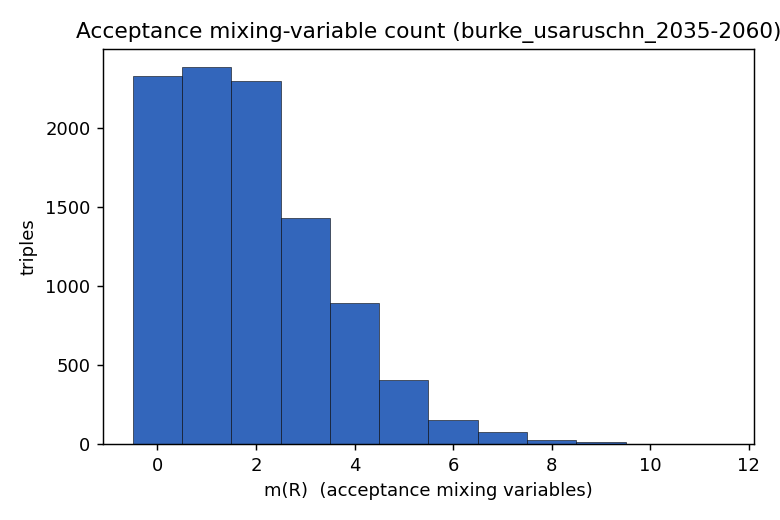
\includegraphics[width=0.6\textwidth]{measurements/plot_m_distribution.png}
\caption{Distribution of the acceptance mixing dimension $m(R)$ over $10^4$ random
triples (median $2$, max $14$; $23\%$ have $m=0$). This is the cheap a-priori
predictor of per-label cost: solve time rises super-linearly in $m$.}
\label{fig:mdist}
\end{figure}

\subsection{Component 2: the proposal-support count \texorpdfstring{$r$}{r}}
\label{sec:comp-r}
\paragraph{What $r$ is.} For one $(\text{proposer},\text{state})$ cell the
\emph{proposal support} is the set of feasible targets that receive positive
probability (a singleton = pure proposal; size $\geq2$ = the proposer mixes). The
proposer can only mix over targets that are \emph{co-maximal} in expected value, which
generically means targets it ranks \emph{tied} at the top. Counting non-empty subsets
of the top-tier-tied feasible targets and multiplying over the $15$ cells gives
\[
r(R)=\prod_{\text{cells}}\big(2^{t}-1\big),\qquad t=\#\{\text{feasible targets at the proposer's best tier}\}.
\]
With the feasibility counts $(4,3,3,3,4)$ per proposer (the adjacency ``diamond'' of
Section~\ref{sec:adjacency}), a cell with no top-tie has $t{=}1$ and contributes a
factor $1$ (pure, nothing to enumerate); a cell with a $k$-way top-tie contributes
$2^k-1$. So $r$ is $1$ exactly when every proposer has a strict best move, and grows
only where $R$ supplies ties.

\paragraph{Distribution.} Over $2\times10^5$ triples, $r$ is \textbf{extremely
heavy-tailed}: median $27$, $p_{90}=2{,}835$, $p_{99}=5.8\times10^5$,
$p_{99.9}=3.7\times10^7$, mean $1.3\times10^6$, maximum $1.2\times10^{11}$. The mean
sits far above the median and grows with sample size --- the signature of a
distribution whose total is dominated by its largest few values.

\paragraph{Caveat (it is itself an upper bound on realisable supports).} $r(R)$ counts
\emph{candidate} supports; a support is truly realisable only if its targets can be
made exactly EV-tied, an extra equation most candidates fail. So $r$ over-counts the
realisable supports. But for a \emph{complete} (waterproof) search this does not
reduce the work: one cannot skip a candidate without testing it, so all $r(R)$
candidates must be handled regardless. (The often-quoted $4.6\times10^{14}$
all-subsets-of-all-feasible figure is a still looser bound and is not the work.)


\paragraph{The feasible-target vector $(4,3,3,3,4)$, and why it is structural.} How
many targets each cell has is the per-proposer vector
$\big(|\mathcal F(i,\empt)|,\dots,|\mathcal F(i,\state{CHNRUSUSA})|\big)=(4,3,3,3,4)$
in state order $\big(\empt,\state{CHNRUS},\state{CHNUSA},\state{RUSUSA},
\state{CHNRUSUSA}\big)$ --- read straight off the adjacency diamond of
Section~\ref{sec:adjacency} ($4$ from \empt{} and from the grand coalition, $3$ from
each pair).

\begin{remark}[This vector is structural, not instance-specific]
\label{rem:structural}
$(4,3,3,3,4)$ comes \emph{only} from the state set and \texttt{adjacent\_step}, not
from the payoffs of Figure~\ref{fig:table}. Hence: (a) it is identical for all three
proposers; (b) it is identical for every one of the $541^3$ triples (a triple fixes
value rankings, not feasible sets); and (c) it is identical for every $n=3$
power-threshold \texttt{adjacent\_step} table --- verified directly on
\texttt{burke\_usaruschn}, \texttt{kalkuhl\_usachnnde}, \texttt{andreoni\_usachnnde}
(all give $(4,3,3,3,4)$). Only the payoffs, hence the equilibria, differ; the
feasibility skeleton is shared.
\end{remark}

The number of candidate supports per cell is $2^{|\mathcal F|}-1$ (each feasible target
independently in/out of the support gives $2^{|\mathcal F|}$ subsets; subtract the
empty one, since a proposer must always propose \emph{something}, at minimum
``stay''). So $(4,3,3,3,4)\mapsto(15,7,7,7,15)$; e.g.\ USA in \state{CHNRUS} has the
$7$ non-empty subsets of $\{\empt,\state{CHNRUS},\state{CHNRUSUSA}\}$ (three pure, three
two-way mixes, one three-way mix).

\begin{figure}[h]
\centering
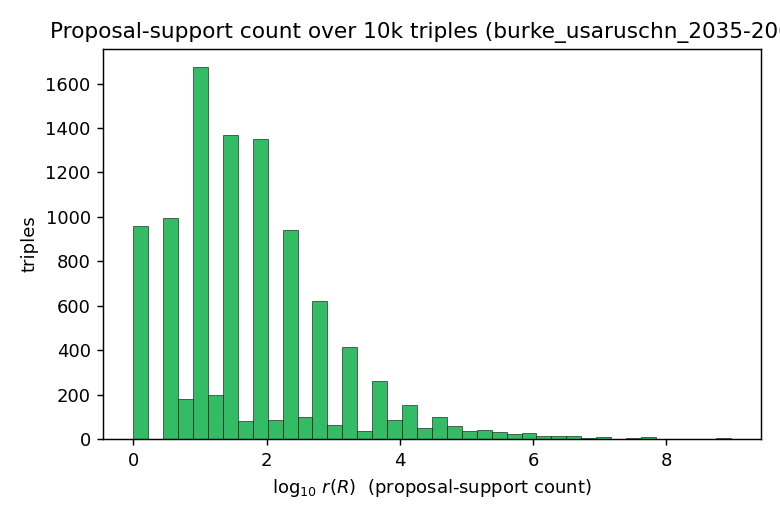
\includegraphics[width=0.6\textwidth]{measurements/plot_r_distribution.png}
\caption{Distribution of $\log_{10}r(R)$ over $10^4$ triples. Heavy-tailed: most
labels are tiny ($9.6\%$ have $r=1$, median $27$) but the tail reaches $r\sim10^{11}$,
which is what makes the full search's total ill-conditioned (\S\ref{sec:joint}).}
\label{fig:rdist}
\end{figure}

\subsection{Interaction: the joint distribution of \texorpdfstring{$r$}{r} and \texorpdfstring{$m$}{m}}
\label{sec:joint}
The two components are not independent --- both are manufactured by ties in $R$, so a
tie-rich triple tends to have \emph{both} a high $m$ and a high $r$. Measured
(\texttt{joint\_analysis.py}, $N=2\times10^5$):
\begin{itemize}[nosep]
\item rank correlation $\rho_{\text{Spearman}}(r,m)=0.44$ (clear positive coupling);
\item median $r$ rises steeply with $m$: $9$ at $m{=}0$, $27$ at $m{=}2$, $567$ at
$m{=}5$, $15{,}309$ at $m{=}8$, $583{,}443$ at $m{=}10$ (Figure~\ref{fig:joint}).
\end{itemize}
Because the expensive-in-$r$ labels are also the expensive-in-$c(m)$ labels, the
\emph{product} $r\cdot c(m)$ concentrates ferociously. Sorting labels by cost:
\begin{center}
\begin{tabular}{lrr}
\toprule
share of labels & \% of \emph{acceptance} cost ($c(m)$) & \% of \emph{full} cost ($r\,c(m)$)\\
\midrule
top $1\%$    & $74.0\%$ & $99.998\%$\\
top $0.1\%$  & $18.7\%$ & $99.82\%$\\
top $0.01\%$ & $2.9\%$  & $97.4\%$\\
single most expensive (sampled) label & $0.14\%$ & $\mathbf{79.2\%}$\\
\bottomrule
\end{tabular}
\end{center}
The full-cost column answers the natural question ``does the top $1\%$ really carry
$100\%$, and the rest $0\%$?'' --- not literally: the top $1\%$ carry $99.998\%$ and
the remaining $99\%$ carry the small but non-zero remainder, $0.0024\%$ (these are
real labels with real, modest cost). What is true is the extreme concentration: a
\emph{single sampled} label carries $79\%$ of the sample's full cost. And the genuine
worst label is far beyond any sample --- it is the fully-tied triple of
Section~\ref{sec:worked}, with $r=4.6\times10^{14}$, whose cost alone is
$\sim3.7\times10^{8}$ years. The acceptance cost is also concentrated (top $1\%$
$=74\%$) but far less pathologically.

\begin{figure}[h]
\centering
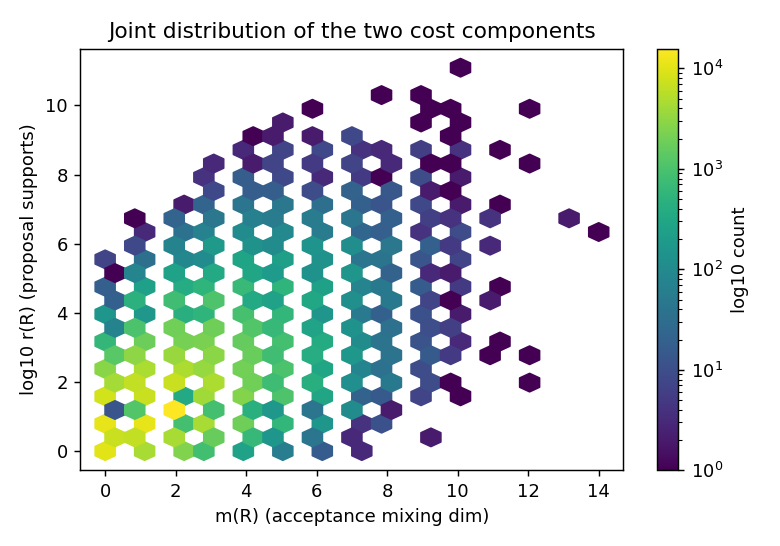
\includegraphics[width=0.66\textwidth]{measurements/plot_joint_r_m.png}
\caption{Joint distribution of the two cost components ($\log_{10}r$ vs.\ $m$) over
$2\times10^5$ random triples. They are positively coupled: tie-rich triples sit in the
upper-right (both large), and that corner --- a vanishing fraction of labels ---
carries essentially all of the full-search cost.}
\label{fig:joint}
\end{figure}

\subsection{Putting it together: the expected duration}
\label{sec:duration}

\paragraph{Acceptance-class search: known with high confidence (direct measurement).}
With $r{=}1$ the cost is $\sum_R c(m(R))$, and this we can state with confidence for
two independent reasons. First, the cost is \emph{statistically stable}: $\mathbb{E}[c]
=0.21$\,s with only $6.5\%$ chunk-to-chunk scatter (\S\ref{sec:joint}). Second --- and
most faithfully --- we did not model it but \textbf{ran the actual exact solver on a
random sample of $10^4$ labels} and extrapolated (\texttt{direct\_sweep\_timing.py},
$1{,}891$\,s wall, per-label mean $0.19$\,s, median $0.0015$\,s):
\begin{center}
\begin{tabular}{lrrr}
\toprule
sweep (cheapest-first) & core-hours & on 14 workers & on 134 workers\\
\midrule
cheapest $50\%$ of labels   & $12$     & $0.9$\,h   & $0.1$\,h\\
cheapest $90\%$ of labels   & $323$    & $23$\,h    & $2.4$\,h\\
cheapest $99\%$ of labels   & $2{,}356$ & $7.0$ days & $0.7$ days\\
cheapest $99.9\%$ of labels & $7{,}435$ & $22.1$ days & $2.3$ days\\
\textbf{complete ($100\%$)} & $\mathbf{8{,}315}$ & $\mathbf{24.7\ \text{days}}$ & $\mathbf{2.6\ \text{days}}$\\
\bottomrule
\end{tabular}
\end{center}
So the acceptance-class certified search for \texttt{burke\_usaruschn} is
\textbf{$\approx25$ days on 14 workers} ($\approx2.6$ days on the 134-core farm),
measured directly and consistent with the component estimate ($\sim27$ days) of
Section~\ref{sec:duration}'s category table. The complete and $99.9\%$ rows are mild
\emph{lower} bounds ($47$ of the $10^4$ labels hit a $20$\,s measurement cap), which a
faster exact high-$m$ solver removes; the cheapest $99\%$ never touch the cap and are
exact. Cheapest-first, predicting $m$ for free, $90\%$ of the entire search is done in
under a day on 14 workers and the cost sits in the small tail.

\paragraph{Full proposal-mixing search: what we \emph{can} estimate, and why the
complete total is still out of reach.} An earlier draft called the full cost
``unmeasurable'' --- that was wrong, and worth correcting precisely, because both
factors of $C_{\text{full}}(R)=r(R)\,c(m(R))$ are obtainable from cheaply-gathered
data: $r(R)$ is a \emph{deterministic structural count} (no solving), and $c(m)$ is
\emph{measured}. Consequently:
\begin{itemize}[nosep]
\item \textbf{Any single label's full cost is computable} --- including the worst one.
The most expensive label is not a mystery to be sampled: it is the fully-tied triple
(Section~\ref{sec:worked}), with $r=4.6\times10^{14}$ and $c(m)\approx25$\,s, i.e.\
$\sim10^{16}$\,s $\approx 3.7\times10^8$ years \emph{for that one label}. (One can also
estimate any label's $c_{\text{support}}$ directly by solving a handful of its
supports and multiplying by its known $r$ --- so even ``sampling within a label''
works; nothing is fundamentally unknowable pre-computation.)
\item \textbf{The cheapest-fraction costs are computable and well-behaved} (table
below): for the bulk of labels $r$ and $c$ are modest and well-sampled.
\item \textbf{Only the \emph{complete} total is statistically awkward to estimate by
random sampling}, because it is dominated by the extreme tie-rich tail (in a $10^5$
sample a single label already holds $79\%$ of the cost; ten-way chunk means scatter
$223\%$ vs.\ $6.5\%$ for acceptance). But we do not need a precise total: the
\emph{single} fully-tied label already costs $\sim3.7\times10^8$ years, so the complete
full search is infeasible by brute force regardless --- a \emph{computed} conclusion,
not an unmeasured one.
\end{itemize}

\paragraph{Full-model budget table: ``what share of labels fits in a given budget?''}
Because per-label full costs are computable, we can answer the planning question
directly. Ordering labels cheapest-first by $r(R)\,c(m(R))$ and extrapolating to all
$541^3$:
\begin{center}
\begin{tabular}{lrrr}
\toprule
cheapest share of labels (full model) & core-hours & on 14 workers & on 134 workers\\
\midrule
$50\%$   & $231$         & $0.7$ days      & $0.07$ days\\
$90\%$   & $1.0\times10^5$ & $310$ days    & $32$ days\\
$99\%$   & $4.2\times10^7$ & $1.2\times10^5$ days & $1.3\times10^4$ days\\
$99.9\%$ & $3.2\times10^9$ & $9.4\times10^6$ days & $9.8\times10^5$ days\\
\bottomrule
\end{tabular}
\end{center}
This is the full-model analogue of the acceptance table above (Figure~\ref{fig:lorenz}
plots both concentration curves). The message: a \emph{partial} full search is genuinely
feasible up to a point --- the cheapest $\sim50\%$ of full-mixing labels finish in
under a day on 14 workers, and one could push perhaps to the cheapest $\sim70$--$80\%$
in a week or two --- but the curve then turns sharply vertical (cheapest $90\%$ already
$\sim10$ months on 14 workers), and the last fraction is dominated by the tie-rich
tail and the single fully-tied label. So a budget buys a well-defined \emph{share} of
the full model, but never the complete sweep.

\paragraph{What this means.} The two objects are sharply different. The
\textbf{acceptance-class} search is a real, runnable, $\sim$\,month-scale (14-worker)
job whose time we know to $\sim$$10\%$. The \textbf{full} search admits a feasible
\emph{partial} run (cheapest tens of percent) but never a complete one; its cost is
concentrated on $<0.01\%$ of labels --- a handful of tie-rich orderings led by the
fully-tied triple --- so full feasibility reduces to whether that tail can be tamed: a
\emph{structural} reduction proving the extreme-tie labels cannot host (or cannot need
to enumerate) so many supports. That is a mathematical question
(Section~\ref{sec:scope}), not a matter of more cores.


\paragraph{Acceptance-class time by case category.} Binning all $541^3$ labels by $m$
and weighting by the measured frequency (\texttt{measure\_total\_time.py}):
\begin{center}
\begin{tabular}{lrrrr}
\toprule
category & \% of labels & core-hours & on 14 workers & on 134 workers\\
\midrule
easy ($m\leq2$)       & $69.4\%$ & $28$      & $2.0$\,h  & $0.2$\,h\\
medium ($m{=}3$--$5$) & $27.7\%$ & $1{,}378$ & $98$\,h   & $10$\,h\\
hard ($m{=}6$--$8$)   & $2.85\%$ & $5{,}907$ & $422$\,h  & $44$\,h\\
extreme ($m\geq9$)    & $0.13\%$ & $1{,}739$ & $124$\,h  & $13$\,h\\
\midrule
\textbf{total}        & $100\%$  & $\mathbf{9{,}052}$ & $\mathbf{\sim27\ \text{days}}$ & $\mathbf{\sim2.8\ \text{days}}$\\
\bottomrule
\end{tabular}
\end{center}
The easy $69\%$ finish in $\sim2$ hours; $>85\%$ of the time is in the hard/extreme
tail ($m\geq6$, $<3\%$ of labels). Figure~\ref{fig:lorenz} shows the cumulative
cost-concentration (``Lorenz'') curves for both objects.

\begin{figure}[h]
\centering
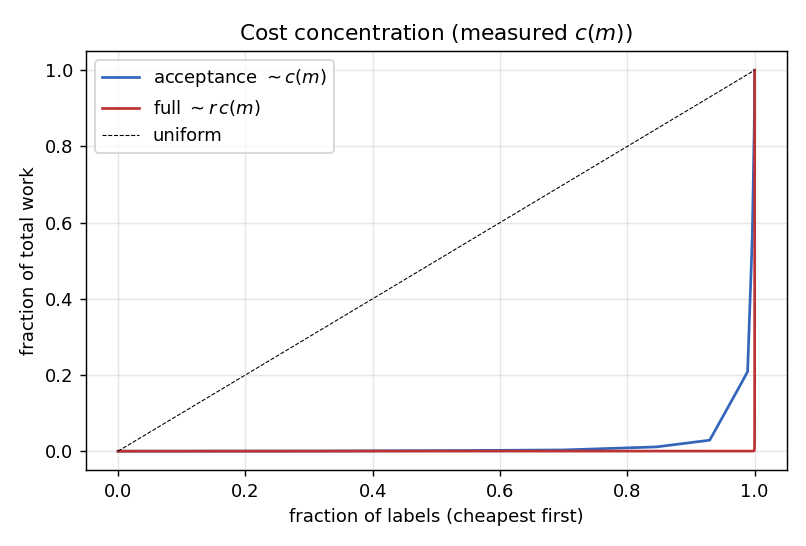
\includegraphics[width=0.62\textwidth]{measurements/plot_lorenz.png}
\caption{Cost concentration, cheapest-first, under the measured $c(m)$. $x$: fraction
of labels processed; $y$: fraction of total work cleared. The acceptance curve (blue)
is concentrated but workable; the full curve (red) hugs the corner --- a single label
holds $73\%$ of its cost (\S\ref{sec:joint}).}
\label{fig:lorenz}
\end{figure}

\section{Scope of the guarantee}
\label{sec:scope}
We distinguish three regimes, because they have very different costs and the
distinction has repeatedly tripped us up:
\begin{description}
\item[Acceptance mixing, fixed proposals.] Enumerate $541^3$ labels; per label the
proposal is pinned by a deterministic rule --- concretely, each proposer is taken to
propose its best-ranked \emph{approvable} target (e.g.\ if USA in \state{CHNRUS}
ranks \state{CHNRUSUSA} top among approvable moves, it proposes \state{CHNRUSUSA}
purely) --- and only acceptances mix. Certified and feasible with a fast backend.
\emph{Limitation:} if the equilibrium needs the proposer itself to mix (a genuinely
two-element proposal support), this regime cannot represent it.
\item[Full mixing (acceptances \emph{and} proposals).] The regime ``that truly
matters.'' Per label the complementarity solve must also resolve proposal mixing.
Certified; feasibility hinges on $r\cdot c$, whose joint distribution and totals are analysed in Section~\ref{sec:joint}--\ref{sec:duration}.
\item[Find-one, not certified.] Methods such as perturbation/homotopy continuation
that return \emph{a} full-mixing equilibrium without a completeness guarantee. Useful
as an independent cross-check and as a fast route to a first solution.
\end{description}

\section{What this document commits to, and what remains open}
\label{sec:open}
The strategy is: \emph{enumerate the $541^3$ weak-order triples; for each, eliminate
irrelevant variables, build the exact polynomial feasibility system of
Section~\ref{sec:perlabel}, and solve it with a certified backend that captures
isolated and positive-dimensional solutions.} This is correct (it cannot miss within
its declared regime) and is validated on a known reduced game. The decisions still to
be made, and to be settled by measurement before committing months of compute, are:
\begin{enumerate}[nosep]
\item the per-label realisable-active-set count $r$ and solve cost $c$ with a fast
backend (this fixes the total cost of Equation~\eqref{eq:components});
\item whether acceptance-only certification already resolves the running instance (if
it certifies \emph{no} acceptance-only equilibrium, that is itself the theorem
``\texttt{burke\_usaruschn} requires proposal mixing'');
\item the choice of certified backend (\texttt{msolve} vs.\ certified homotopy) and
the distributed harness across the available cores.
\end{enumerate}


\appendix
\section{Peripheral sub-analyses (not load-bearing)}
\label{app:peripheral}
These items are not essential to the argument --- the headline costs of
Section~\ref{sec:counting} do not rest on them --- but they are the hard numbers
behind some statements, recorded for completeness.

\subsection{A loose upper bound: ``conceivable combinations''}
\label{app:upperbound}
One can bound the search by treating each cell's proposal support as a free,
independent choice. With supports $(15,7,7,7,15)$ per proposer, a full \emph{support
profile} (one choice for all $15$ cells) numbers $15\cdot7\cdot7\cdot7\cdot15=77{,}175$
per proposer, so $77{,}175^3\approx4.6\times10^{14}$ profiles, and
$\times541^3\approx7.3\times10^{22}$ ``labels''; restricting to pure proposals still
leaves $432^3\times541^3\approx1.3\times10^{16}$.

This arithmetic is correct as a count of \emph{conceivable} combinations, but it is
\emph{not} the work and is not a factor in any total. Proposals are not free: given a
triple and the acceptance mixing, the proposer's $\mathrm{EV}$-optimal target is
determined, so almost all $4.6\times10^{14}$ profiles are immediately inconsistent and
never formed. The work is governed instead by the \emph{realisable} support count
$r(R)$ of Section~\ref{sec:comp-r} (median $27$), which is what enters the totals. We
record $7.3\times10^{22}$ only to retire it.

\subsection{Variable elimination and realisable supports}
\label{app:elimination}
Two reductions keep the per-label system small. (i) \emph{Variable elimination}: a
free acceptance variable on a transition no proposer ever proposes never enters $P$,
hence not $V$, hence no equation --- it is dropped; only acceptances on proposed
transitions remain. (ii) \emph{Few indifference equations}: their number is the total
tied-group size minus the number of groups, summed over players --- at most $S-1=4$
per player ($\leq12$ total), usually far fewer. Together these are why, despite up to
$\sim35$ raw mixing contexts, the effective system at a typical triple is tiny.

\subsection{Summary of the key quantities}
\label{app:summary}
\begin{center}
\begin{tabular}{lrl}
\toprule
quantity & value & status\\
\midrule
weak orders per player $a(5)$ & $541$ & exact\\
weak-order triples $541^3$ & $1.58\times10^8$ & exact (outer loop)\\
strict-order triples $120^3$ & $1.73\times10^6$ & exact (no-ties subset)\\
feasible targets / state & $(4,3,3,3,4)$ & exact (adjacency; \S\ref{sec:comp-r})\\
candidate supports / cell & $(15,7,7,7,15)$ & exact\\
mixing dim $m(R)$ & median $2$, max $14$ & measured\\
solve cost $c(m)$ & $0.002$\,s$\to$$18.6$\,s ($m{:}2{\to}8$) & measured; super-linear\\
support count $r(R)$ & median $27$, mean $1.3\times10^6$, max $1.2\times10^{11}$ & measured; heavy-tailed\\
$\rho_{\text{Spearman}}(r,m)$ & $0.44$ & measured\\
acceptance total (14w) & $\sim27$ days & measured, stable ($6.5\%$)\\
full total (14w) & $\sim6\times10^9$ days & $\Sigma r c$; unstable, infeasible\\
\bottomrule
\end{tabular}
\end{center}
\end{document}
